\documentclass{beamer}

% Beamer style
%\usetheme[secheader]{Madrid}
\usetheme{CambridgeUS}
\usecolortheme[rgb={0.65,0.15,0.25}]{structure}
%\usefonttheme[onlymath]{serif}
\beamertemplatenavigationsymbolsempty
%\AtBeginSubsection

% Packages
%\usepackage[french]{babel}
\usepackage[latin1]{inputenc}
\usepackage{color}
\usepackage{dsfont, stmaryrd}
\usepackage{amsmath, amsfonts, amssymb}
\usepackage{stmaryrd}
\usepackage{epsfig}
\usepackage{/media/donnees/LATEX/astats}
%\usepackage[all]{xy}
\usepackage{graphicx}

% Commands
\definecolor{darkred}{rgb}{0.65,0.15,0.25}
\definecolor{darkgreen}{rgb}{0,0.4,0}
\newcommand{\emphase}[1]{\textcolor{darkred}{#1}}
%\newcommand{\emphase}[1]{\textcolor{black}{#1}}
\newcommand{\paragraph}[1]{\textcolor{darkred}{#1}}
\newcommand{\refer}[1]{\textcolor{blue}{\sl \cite{#1}}}
\newcommand{\Refer}[1]{\textcolor{blue}{\sl #1}}
\newcommand{\newblock}{}

% Symbols
\newcommand{\Abf}{{\bf A}}
\newcommand{\Bbf}{{\bf B}}
\newcommand{\Beta}{\text{B}}
\newcommand{\betabf}{\text{\mathversion{bold}{$\beta$}}}
\newcommand{\Bcal}{\mathcal{B}}
\newcommand{\BIC}{\text{BIC}}
\newcommand{\dd}{\text{d}}
\newcommand{\Cbf}{{\bf C}}
\newcommand{\dbf}{{\bf d}}
\newcommand{\Dcal}{\mathcal{D}}
\newcommand{\Esp}{\mathbb{E}}
\newcommand{\Ebf}{{\bf E}}
\newcommand{\Ecal}{\mathcal{E}}
\newcommand{\Fbf}{{\bf F}}
\newcommand{\Gcal}{\mathcal{G}}
\newcommand{\Gam}{\mathcal{G}\text{am}}
\newcommand{\Ibb}{\mathbb{I}}
\newcommand{\Ibf}{{\bf I}}
\newcommand{\ICL}{\text{ICL}}
\newcommand{\Cov}{\mathbb{C}\text{ov}}
\newcommand{\Corr}{\mathbb{C}\text{orr}}
\newcommand{\Var}{\mathbb{V}}
\newcommand{\Vsf}{\mathsf{V}}
\newcommand{\pen}{\text{pen}}
\newcommand{\Fcal}{\mathcal{F}}
\newcommand{\Hbf}{{\bf H}}
\newcommand{\Hcal}{\mathcal{H}}
\newcommand{\Jcal}{\mathcal{J}}
\newcommand{\Kbf}{{\bf K}}
\newcommand{\Lcal}{\mathcal{L}}
\newcommand{\Lbf}{{\bf L}}
\newcommand{\Mcal}{\mathcal{M}}
\newcommand{\mbf}{{\bf m}}
\newcommand{\Ncal}{\mathcal{N}}
\newcommand{\Nbf}{{\bf N}}
\newcommand{\Nm}{N(\mbf)}
\newcommand{\Ocal}{\mathcal{O}}
\newcommand{\Obf}{{\bf 0}}
\newcommand{\Omegas}{\underset{s}{\Omega}}
\newcommand{\Pbf}{{\bf P}}
\newcommand{\Pcal}{\mathcal{P}}
\newcommand{\Qcal}{\mathcal{Q}}
\newcommand{\Rbb}{\mathbb{R}}
\newcommand{\Rcal}{\mathcal{R}}
\newcommand{\sbf}{{\bf s}}
\newcommand{\Sbf}{{\bf S}}
\newcommand{\Scal}{\mathcal{S}}
\newcommand{\Ucal}{\mathcal{U}}
\newcommand{\Vcal}{\mathcal{V}}
\newcommand{\Tbf}{{\bf T}}
\newcommand{\ubf}{{\bf u}}
\newcommand{\Ubf}{{\bf U}}
\newcommand{\Wbf}{{\bf W}}
\newcommand{\xbf}{{\bf x}}
\newcommand{\Xbf}{{\bf X}}
\newcommand{\Ybf}{{\bf Y}}
\newcommand{\Zbf}{{\bf Z}}
\newcommand{\pibf}{\text{\mathversion{bold}{$\pi$}}}
\newcommand{\Sigmabf}{\text{\mathversion{bold}{$\Sigma$}}}
\newcommand{\gammabf}{\text{\mathversion{bold}{$\gamma$}}}
\newcommand{\mubf}{\text{\mathversion{bold}{$\mu$}}}
\newcommand{\nubf}{\text{\mathversion{bold}{$\nu$}}}
\newcommand{\Thetabf}{\text{\mathversion{bold}{$\Theta$}}}
\newcommand{\thetabf}{\text{\mathversion{bold}{$\theta$}}}
\newcommand{\BP}{\text{BP}}
\newcommand{\EM}{\text{EM}}
\newcommand{\VEM}{\text{VEM}}
\newcommand{\VBEM}{\text{VB}}
\newcommand{\cst}{\text{cst}}
\newcommand{\obs}{\text{obs}}
\newcommand{\ra}{\emphase{$\rightarrow$~}}
\newcommand{\QZ}{Q_{\Zbf}}
\newcommand{\Qt}{Q_{\thetabf}}

% Directory
\newcommand{\fighd}{../Figures}
\newcommand{\figSimHMM}{../Figures/CGH-HMM-sim/CGHsim-9}


%====================================================================
\title[Statistics \& Segmentation in Genomics]{Some Statistical
  Models and Algorithms for Change-Point Problems in Genomics}

\author[S. Robin]{S. Robin}

\institute[AgroParisTech / INRA]{UMR 518 AgroParisTech / INRA Applied
  Math \& Computer Sc.\\
  \bigskip
  \begin{tabular}{ccccc}
    
\epsfig{file=../Figures/LogoINRA-Couleur.ps,
    width=2.5cm} & 
    \hspace{.5cm} &
    
\epsfig{file=../Figures/logagroptechsolo.eps,
    width=3.75cm} & 
    \hspace{.5cm} &
    
\epsfig{file=../Figures/logo-ssb.eps,
    width=2.5cm} \\ 
  \end{tabular} \\
  \bigskip
  }

  \date[Stuttgart, 2012]{Statistical and Dynamical Models in Biology and
    Medicine \\ University Stuttgart, October 11-12, 2012}

%====================================================================

%====================================================================
%====================================================================
\begin{document}
%====================================================================
%====================================================================

%====================================================================
\frame{\titlepage
  }

%====================================================================
\frame{\frametitle{Outline} 
  \tableofcontents

  }

%====================================================================
%====================================================================
\section{Biological motivation}
%====================================================================
\frame{\frametitle{Biological (and statistical) motivation}}

%====================================================================
\subsection*{Genomic alterations in cancer cells}
%====================================================================
\frame{\frametitle{Genomic alterations in cancer cells}

  Genomic alterations are associated with (responsible for?) various
  types of cancers.
  
  \begin{tabular}{cc}
    \onslide+<1->{Normal cell} & \onslide+<2->{Tumor cell} \\
    \onslide+<1->{
      \epsfig{file =
        \fighd/KaryotypeCancer-PH.ps, clip=,
        bbllx=325, bblly=676, bburx=468, bbury=780, scale=.9} 
    }
    &
    \onslide+<2->{
      \epsfig{file =
        \fighd/KaryotypeCancer-PH.ps, clip=,
        bbllx=127, bblly=676, bburx=319, bbury=780, scale=.9} 
    }
  \end{tabular}
  
  \onslide+<2->{
    Source: \refer{Hup08}. 
  }
}

%====================================================================
\frame{\frametitle{Array CGH technology: principle}
  
\epsfig{file = ../Figures/principe_CGH.eps, clip=,
  bbllx=0, bblly=41, bburx=700, bbury=478, width=.9\textwidth}
}

%====================================================================
\frame{\frametitle{Segmentation: the basic problem}
  
  %\vspace{-0.5cm}
  \begin{tabular}{cc}
    \begin{tabular}{p{.5\textwidth}}
      \onslide+<1->{
        \paragraph{Data at hand:} for a given individual
        \begin{itemize}
        \item a sequence of \emphase{known positions} along the
          \emphase{reference genome}, labeled as
          \[
          t = 1, 2, \dots, n
          \]
        \item a signal measured \emphase{at each position}
          \[
          Y_t = \text{signal at position $t$}
          \]
        \end{itemize}
        }
    \end{tabular}
    &
    \begin{tabular}{p{.5\textwidth}}
      \hspace{-1cm}
      \begin{overprint}
        \onslide<2-3>
        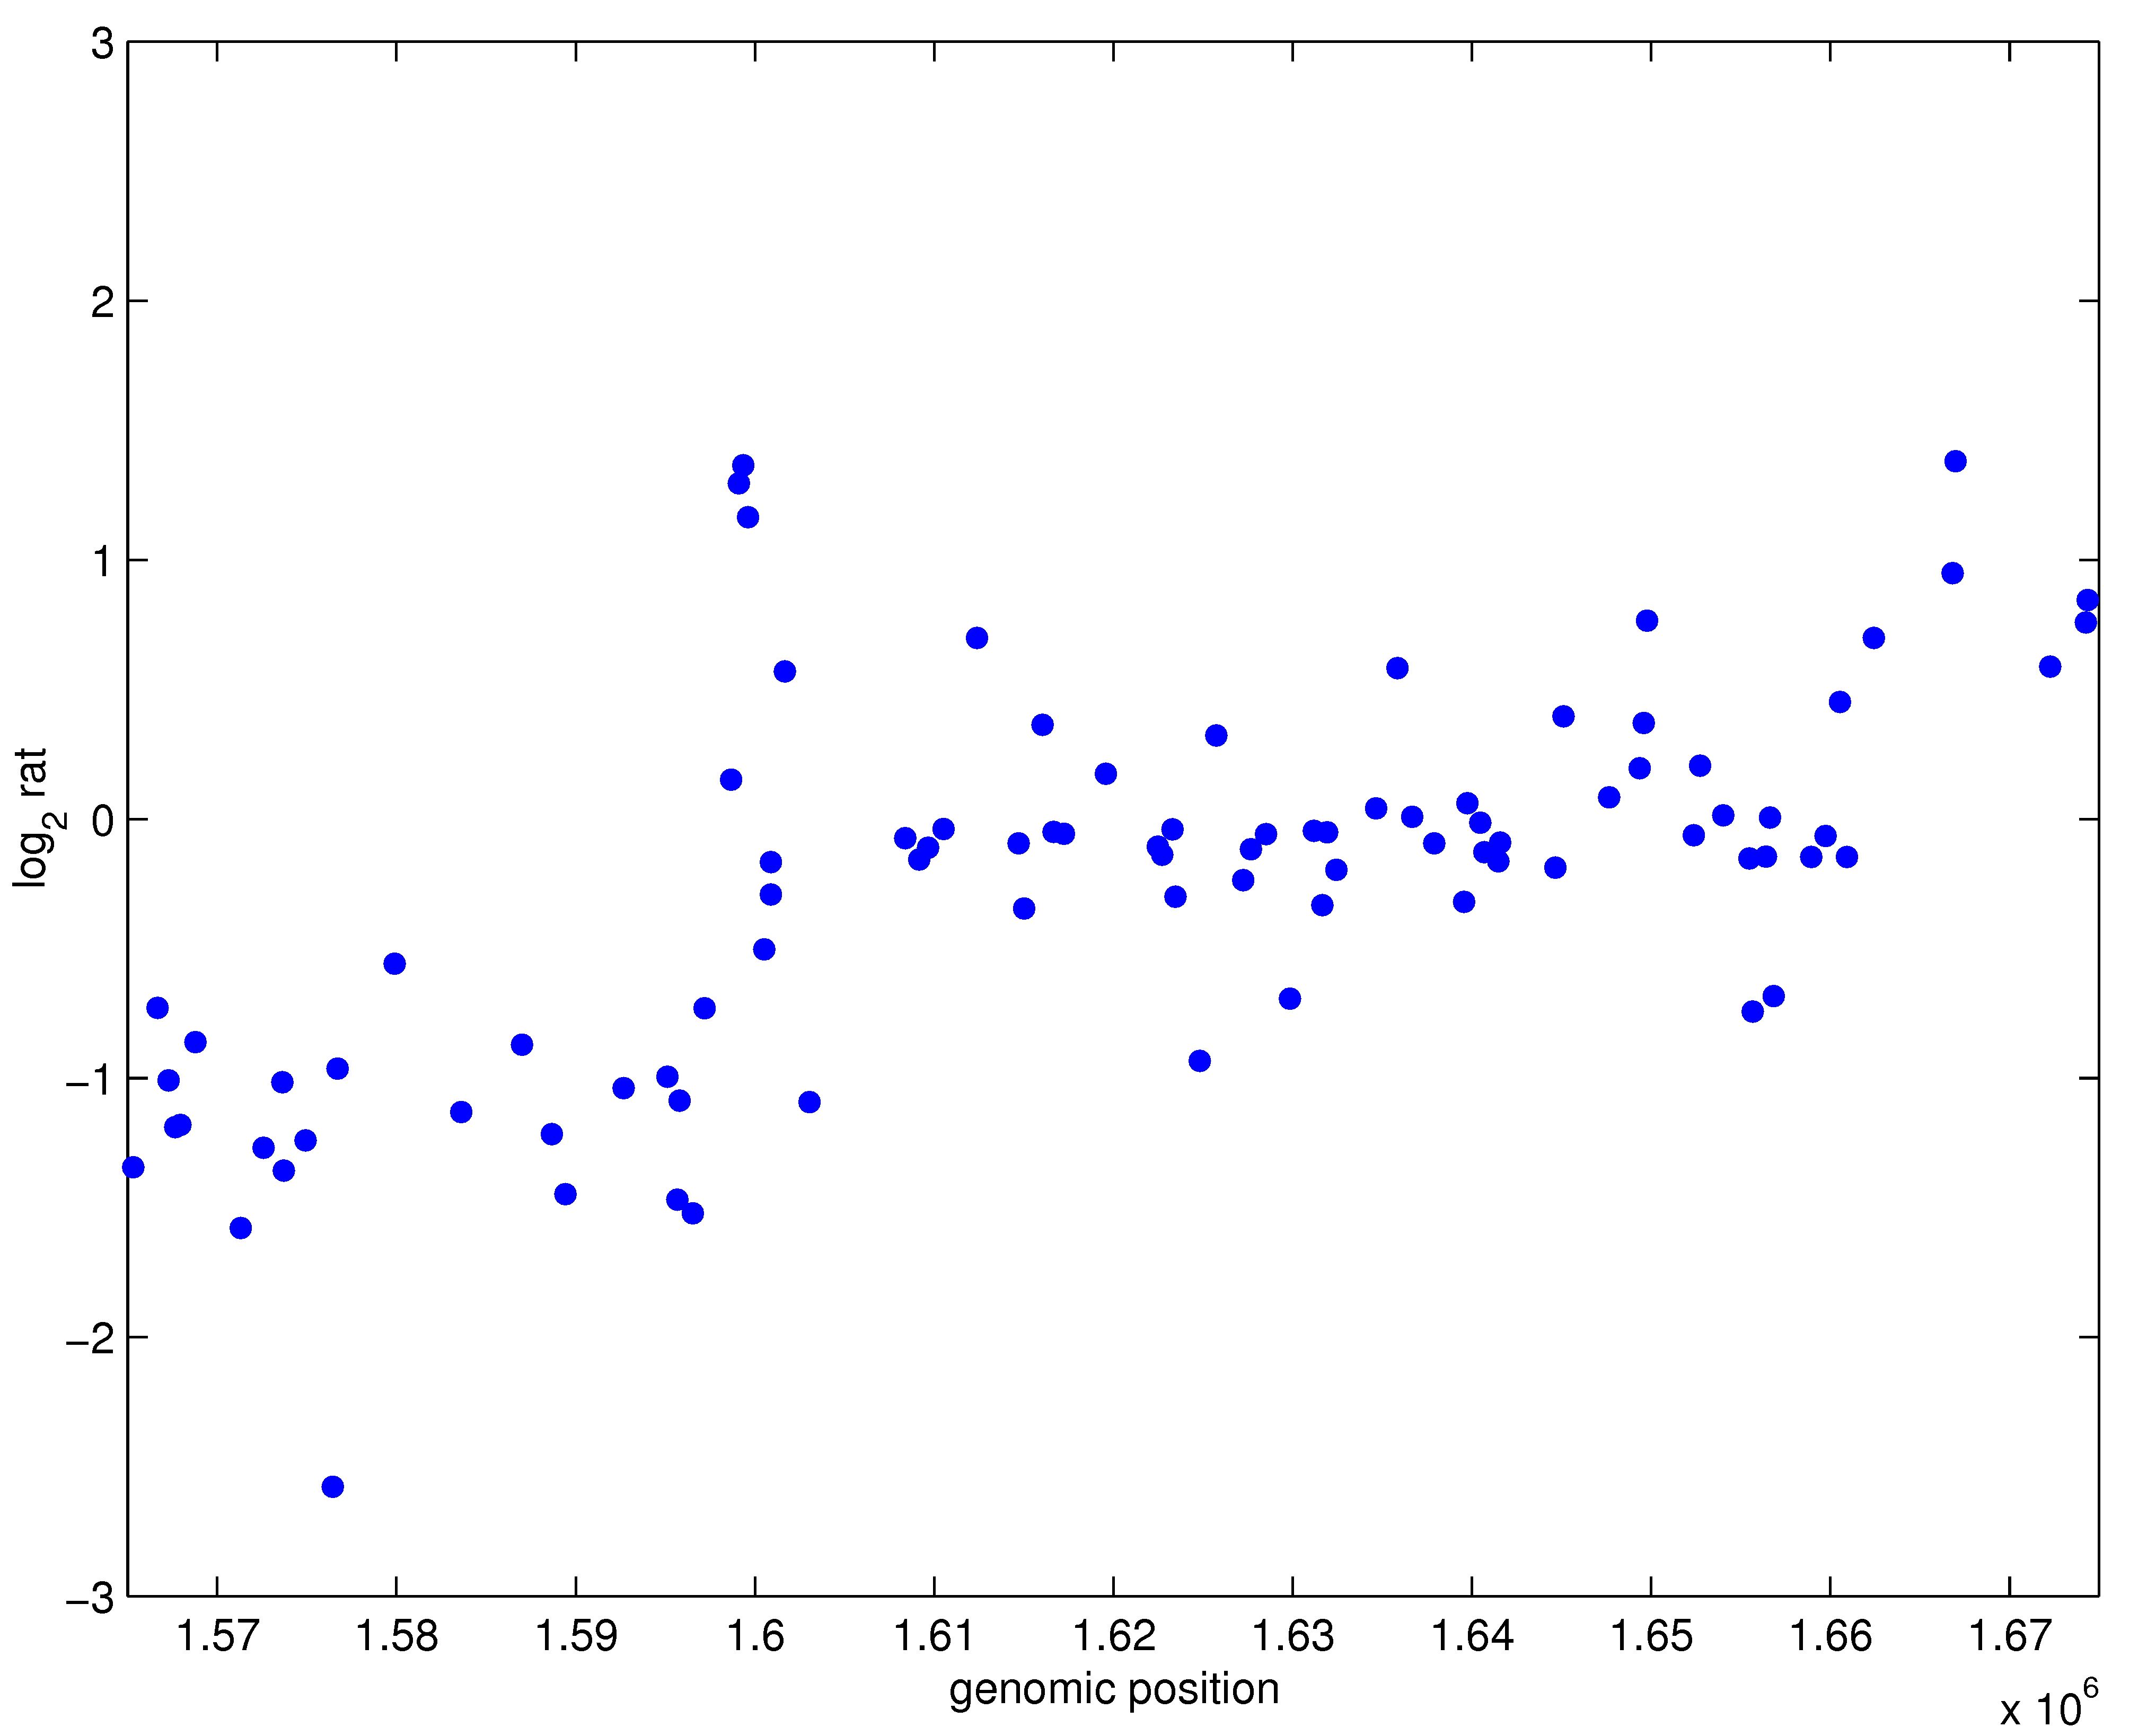
\epsfig{file = ../Figures/raw_profile_example.eps, clip=,
          width=.45\textwidth, height=.5\textheight}  
        \onslide<4>
        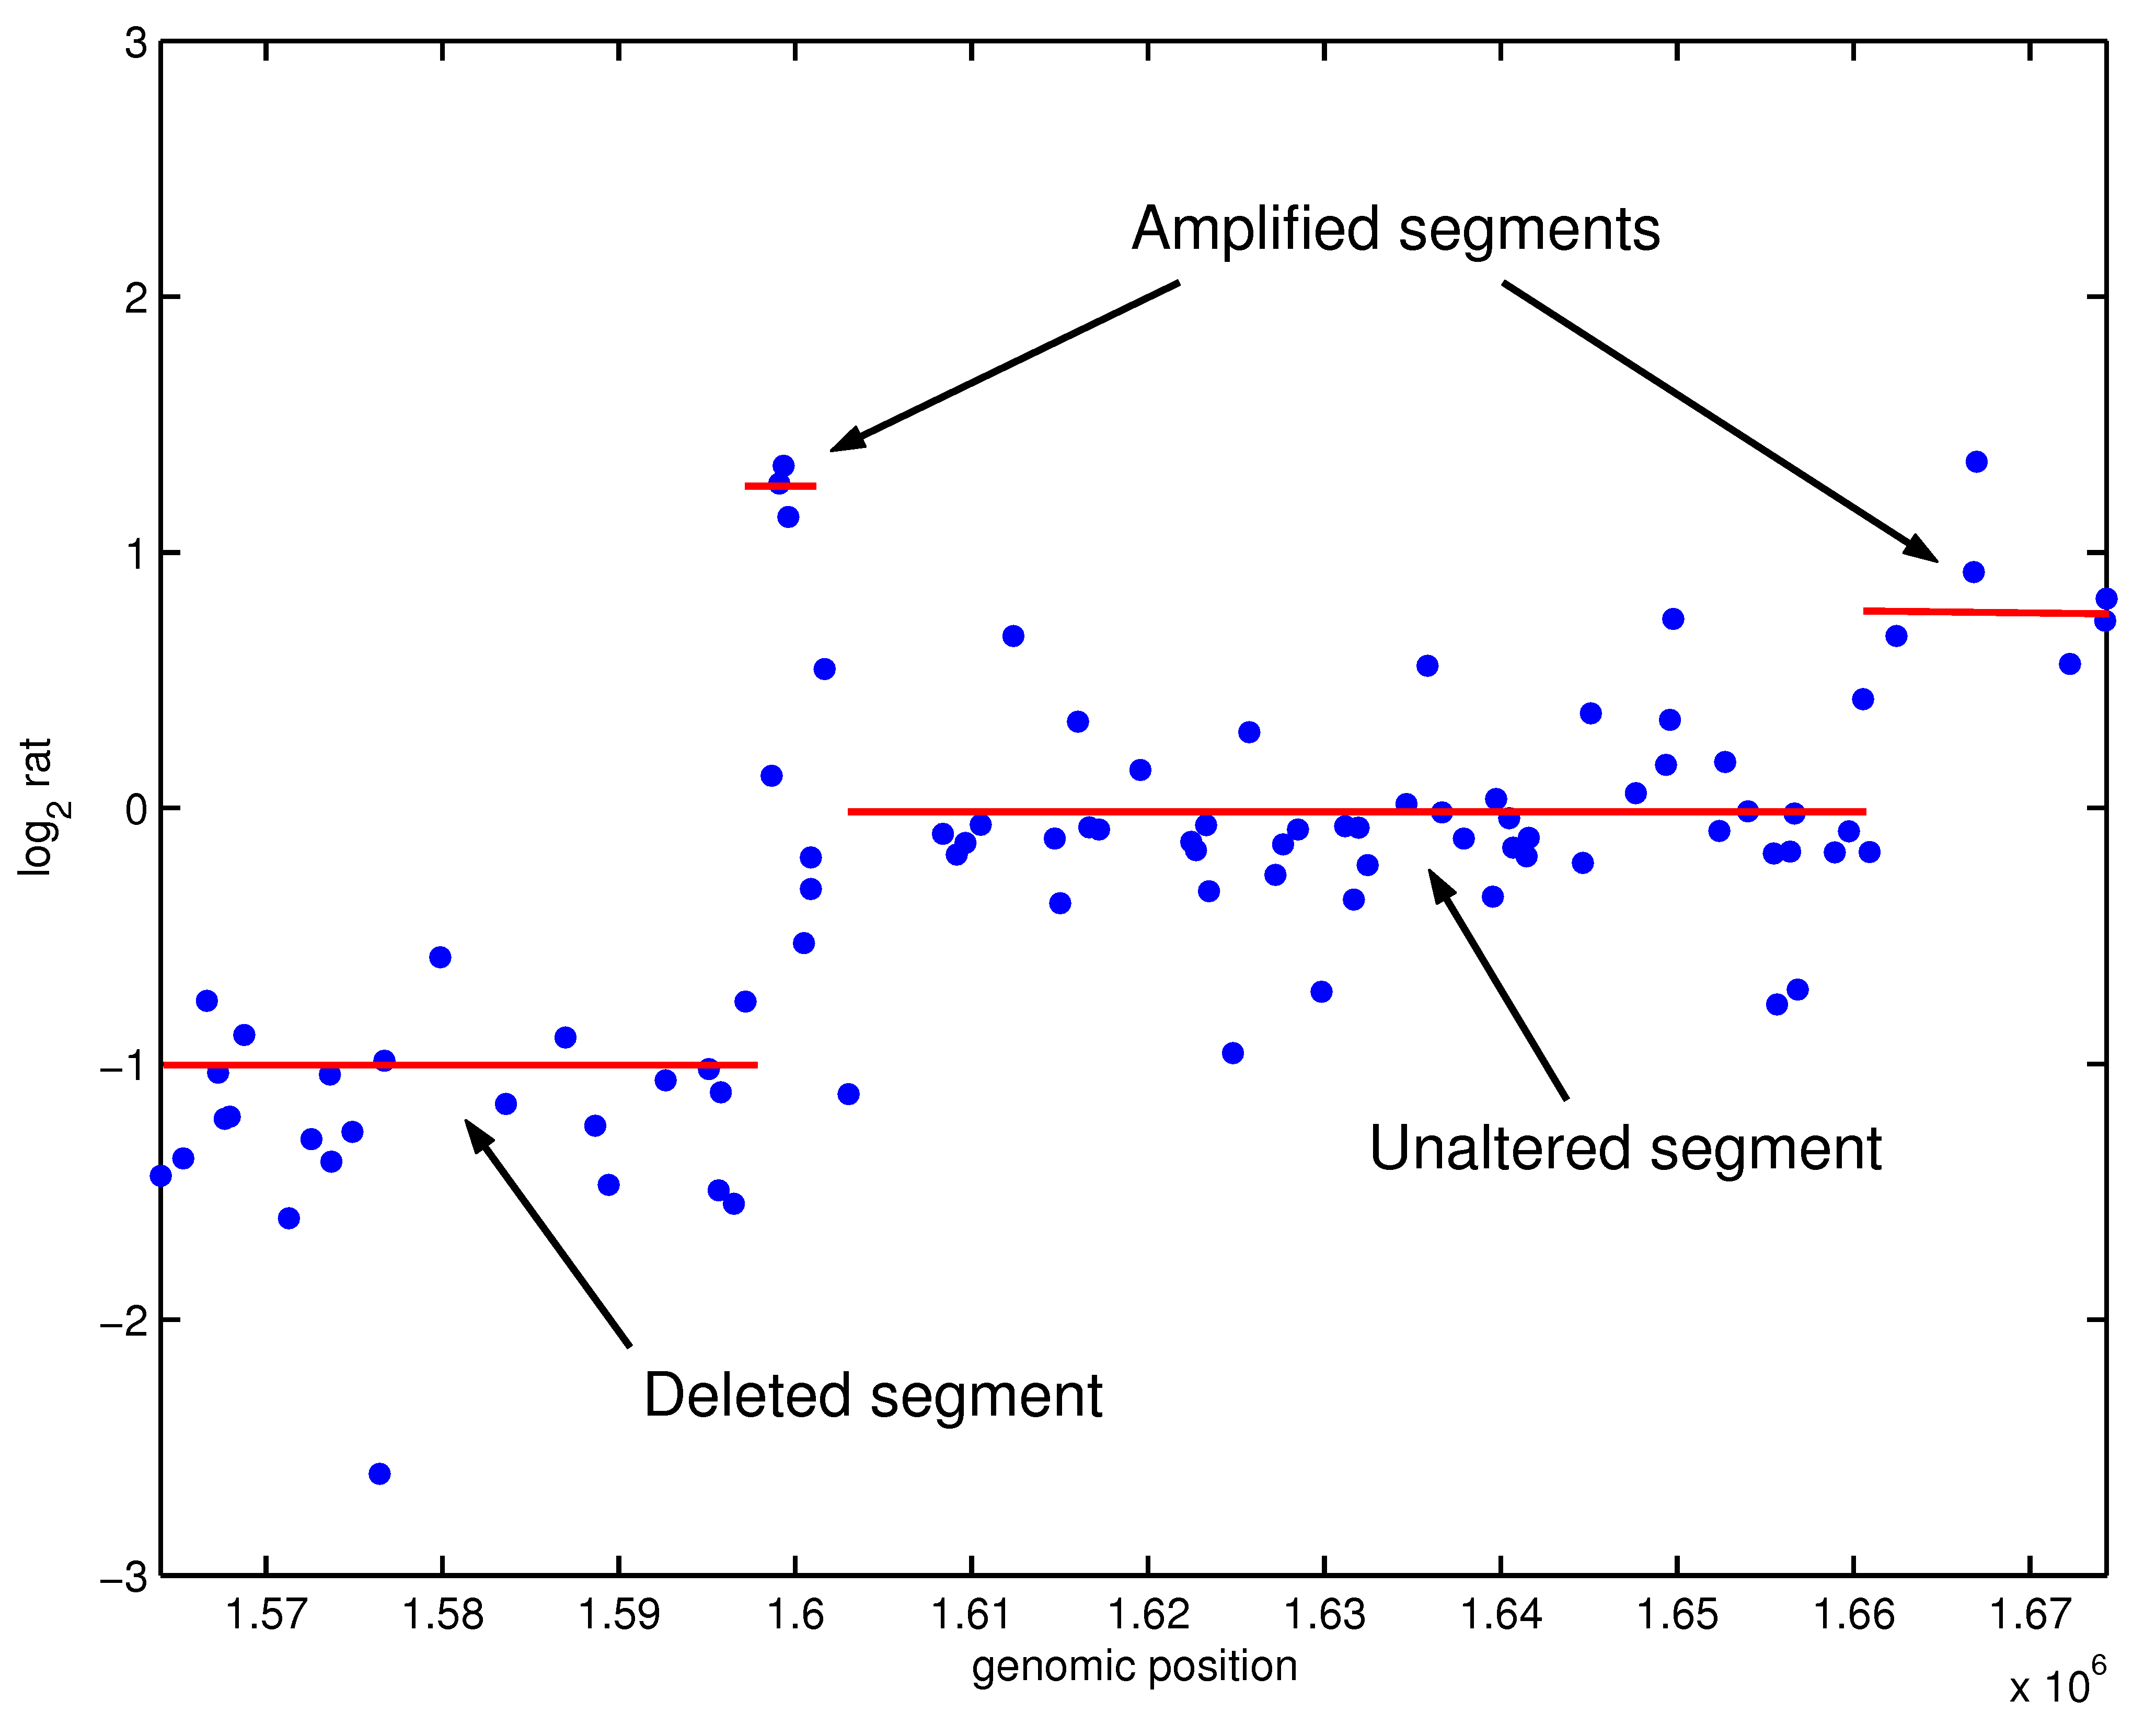
\epsfig{file = ../Figures/profile_example.eps, clip=,
          %bbllx=60, bblly=196, bburx=543, bbury=586}
          width=.45\textwidth, height=.5\textheight}  
      \end{overprint}
    \end{tabular}
  \end{tabular} \\
  \onslide+<3->{
    \begin{eqnarray*}
      Y_t & \propto & f(\text{\emphase{relative copy number} at position }t) \\
      & = & \text{log-fluorescence, sum of the two allele signals for a given
        SNP, etc.}
    \end{eqnarray*}
    }
  }

%====================================================================
\frame{\frametitle{Cancer cell genomic alterations}

  \hspace{-.5cm}
  \begin{tabular}{ccccc}
    \multicolumn{3}{c}{Zoom on CGH profile} & \quad & Karyotype \\
    chrom. 1 & \quad & chrom. 17 \\
    \begin{tabular}{c}
      \epsfig{file = ../Figures/Karyotype-CGH-PH.ps, clip=,
        bbllx=80, bblly=617, bburx=150, bbury=700, height=.5\textheight}
    \end{tabular}
    & &
    \begin{tabular}{c}
      \epsfig{file = ../Figures/Karyotype-CGH-PH.ps, clip=,
        bbllx=270, bblly=617, bburx=300, bbury=700, height=.5\textheight}
    \end{tabular}
    & &
    \begin{tabular}{c}
      \epsfig{file = ../Figures/Karyotype-CGH-PH.ps, clip=,
        bbllx=364, bblly=617, bburx=485, bbury=763, height=.5\textheight}
    \end{tabular}
  \end{tabular}

  \bigskip
  CGH technology gives access to CNV, but does not allow the
  positioning of translocations.  (\refer{Hup08}) }

%====================================================================
\subsection*{Genome annotation}
\frame{\frametitle{Genome annotation}}
%====================================================================
\frame{\frametitle{Genome annotation}

  %\vspace{-0.5cm}
  \begin{tabular}{cc}
    \hspace{-0.5cm}
    \begin{tabular}{p{.45\textwidth}}
      \onslide+<1->{ 
        \paragraph{A bit of biology:} 
        Gene coding sequences are organized in exons / introns.  \\
        ~\\
      }      
      \onslide+<2->{
        \paragraph{RNA-seq:}
        Data provided by 'NGS' should allow to locate precisely the
        exon boundaries. \\
        ~\\
      }      
      \onslide+<3->{
        \paragraph{Reconsidering annotation:}
        Hence the 'official' annotation can be reconsidered. \\
        ~\\~\\~\\~\\~\\~\\~\\~\\~\\~\\~\\
      }
    \end{tabular}
    &
    \hspace{-.5cm}
    \begin{tabular}{p{.5\textwidth}}
      \begin{overprint}
        \onslide<1>
        \epsfig{file=../../../EXPRESSION/EXPOSES/Figures/RNASynth-Gal.ps,
          width=.5\textwidth, height=.75\textheight, clip=} 
        \onslide<2>
        \vspace{1cm}
        RNA-seq counts \\
        ~\\
        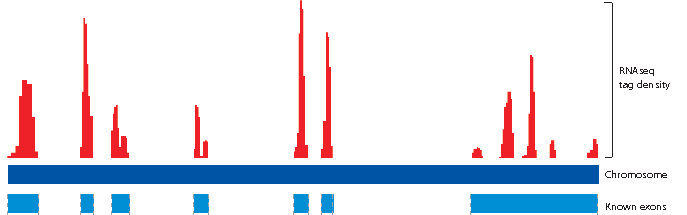
\epsfig{file=../Figures/gb-2008-9-9-234-1.eps,
          width=.5\textwidth, height=.3\textheight, bbllx=0,
          bblly=275, bburx=300, bbury=425, clip=} \\
        ~\\
        Known exons \\
        ~\\
        source: \Refer{genomebiology.com}
        \onslide<3>
        \epsfig{file=../Figures/data.ps, width=.5\textwidth,
          height=.8\textheight, clip=}
      \end{overprint}
    \end{tabular}
  \end{tabular}
}

%====================================================================
\subsection*{Statistical modeling}
%====================================================================
\frame{\frametitle{(Statistical) questions}
  
  \paragraph{Biological questions:}  
  \begin{itemize}
  \item How many change points?
  \item Where are the change points? (How precise is the location?)
  \item Do the change points have the same location in samples $A$
    and $B$?
  \item ...
  \end{itemize}
  
  \bigskip
  \paragraph{Statistical issues:}  
  \begin{itemize}
  \item Statistical modeling
  \item Computational efficiency
  \item Model selection
  \end{itemize}
}

%====================================================================
\frame{\frametitle{Basic segmentation model}

  \begin{tabular}{cc}
    \hspace{-.5cm}
    \begin{tabular}{p{.5\textwidth}}
      \onslide+<2->{\paragraph{Statistical model.} 
        \begin{itemize}
        \item $\text{Signal} = f(\text{Position})$; \\}
        \onslide+<3->{
        \item Breakpoint positions: \\
          $\tau_1, \tau_2, ..., \tau_{K-1};$ \\}
        \onslide+<4->{
        \item Mean signal (e.g. relative copy number) within each interval: \\
          $\theta_1, \theta_2, ..., \theta_K$; \\}
        \onslide+<5->{
        \item Observed signal at time $t$: \\
          independent variables with given means.
        \end{itemize}}
    \end{tabular}
    & 
    \hspace{-1cm}
    \begin{tabular}{c}
      \onslide+<2->{
        \hspace{-6cm}
        \onslide+<3->{if $t \in \textcolor{blue}{r_k}$,} \quad $Y_t$
        \onslide+<5->{$\sim
          \Fcal($}\onslide+<4->{$\textcolor{red}{\theta_k}$}\onslide+<5->{$)$}
        \\}
      \begin{overprint}
        \onslide<2>
%        $\qquad \qquad \;\;\, Y_t =$ \\
        \epsfig{file=../Figures/FigSeg-Budapest-1.eps, clip=,
          angle=270, width=.5\textwidth} 
        \onslide<3>
%        if $t \in \textcolor{blue}{r_k}, \quad Y_t$ \\
        \epsfig{file=../Figures/FigSeg-Budapest-2.eps, clip=,
          angle=270, width=.5\textwidth} 
        \onslide<4>
%        if $t \in \textcolor{blue}{r_k}, \quad Y_t \textcolor{red}{\theta_k}$ \\
        \epsfig{file=../Figures/FigSeg-Budapest-3.eps, clip=,
          angle=270, width=.5\textwidth} 
        \onslide<5->
%        if $t \in \textcolor{blue}{r_k}, \quad Y_t \sim
%        \Fcal(\textcolor{red}{\theta_k})$ \\ 
        \epsfig{file=../Figures/FigSeg-Budapest-4.eps, clip=,
          angle=270, width=.5\textwidth} 
      \end{overprint}
    \end{tabular}
  \end{tabular}

  \onslide+<6->{
    \paragraph{Possible choices for the distribution $\Fcal$:} 
    \begin{itemize}
    \item CGHarray: continuous signal (fluorescence) \ra Gaussian distribution;
    \item NGS: discrete signal (counts) \ra Poisson or negative
      binomial distribution.
    \end{itemize}
  }
}

%====================================================================
\frame{\frametitle{Some specificities}

  \paragraph{Two different types of parameters of the models:}
  \begin{itemize}
  \item Segmentation (change point locations): $T = (\tau_1, \dots,
    \tau_{K-1})$ \\
    \ra discrete parameter;
  \item Distribution parameters (within segment means): $\Theta =
    (\theta_1, \dots, \theta_K)$ \\
    \ra continuous parameter.
  \end{itemize}

  \bigskip\pause
  \paragraph{Segmentation space:}
  \begin{itemize}
  \item The number of possible segmentation $T$ is huge:
    \[
    |\Mcal_K| = \left(\begin{array}{c} n-1 \\ K-1 \end{array} \right);
    \]
  \item The systematic exploration of $\Mcal_K$ is impossible.
  \end{itemize}
  
}

%====================================================================
%====================================================================
\section{Frequentist Inference}
%====================================================================
\frame{\frametitle{Frequentist framework} \pause

  \paragraph{Frequentist principle:} 
  The parameters $T$ and $\Theta$ are \emphase{fixed} and we want to provide
  estimates $\widehat{T}$ and $\widehat{\Theta}$ of their
  \emphase{true values}.

  \bigskip\bigskip\pause
  \paragraph{One classical approach:} Maximum likelihood estimates (MLE)
  \[
  (\widehat{T}, \widehat{\Theta}) = \arg\max_{T, \Theta} \; \log
  P(\Ybf; T, \Theta)
  \]
  where $\Ybf$ stands for the whole data set $\Ybf = (Y_1, \dots, Y_n)$.

  \bigskip\bigskip
  \ra Hybrid optimization problem with both discrete and continuous
  arguments.  
}

%====================================================================
\subsection{One profile}
%====================================================================
\frame{\frametitle{One profile}

  \paragraph{Likelihood.} Thanks to independence assumptions, we have
  \[
  \log P(\Ybf; T, \Theta) = \textcolor{red}{\sum_k}
  \textcolor{blue}{\sum_{t \in r_k} \log P(Y_t ;\theta_k)}.
  \]

  \pause 
  \paragraph{Parameter estimates $\widehat{\Theta}$.} 
  For any segment $r_k$, the MLE of $\theta_k$ is 
  \[
  \widehat{\theta}_k = \arg\max_{\theta_k} \textcolor{blue}{\sum_{t
      \in r_k} \log P(Y_t; \theta_k)},
  \pause
  \qquad \text{e.g. $\widehat{\theta}_k = $ mean within segment $r_k$.}
  \]

  \pause 
  \paragraph{Segmentation estimates $\widehat{T}$.} 
  \begin{itemize}
  \item \pause Finding $\widehat{T}$ is equivalent to a
    \emphase{shortest path} problem where $\sum_{t \in r_k} \log
    P(Y_t; \widehat{\theta}_k)$ is the cost of segment $r_k$.  
  \item \pause Because the cost is \emphase{additive}, this can be
    solve via \emphase{dynamic programming} with time complexity
    $O(Kn^2)$ and space complexity $O(Kn)$.
  \end{itemize}
}\label{Page:ParamInfer}

%====================================================================
\frame{\frametitle{How many change-points?}

  \vspace{-.5cm}
  \begin{tabular}{cc}
    \hspace{-.5cm}
    \begin{tabular}{p{.45\textwidth}}
	  \paragraph{How many segments?}
	  \begin{itemize}
	    \item The number of segments $K$ is not known a priori.
	    \item The fit of the segmentation improves as $K$ 	
		    increases.
	  \end{itemize}
  
	  \bigskip 
	  \paragraph{Penalized likelihood $=$} most common strategy:
	  \[
	  \onslide+<4->{\textcolor{blue}{\widehat{K}} = \arg\min_K}
	  ~\onslide+<2->{- \log P(\Ybf; K)}
	  ~\onslide+<3->{\textcolor{red}{+ \text{pen}(K)}}
	  \]
    \end{tabular}
	&
    \begin{tabular}{p{.5\textwidth}}
	    \begin{overprint}
    	\onslide<2>
	      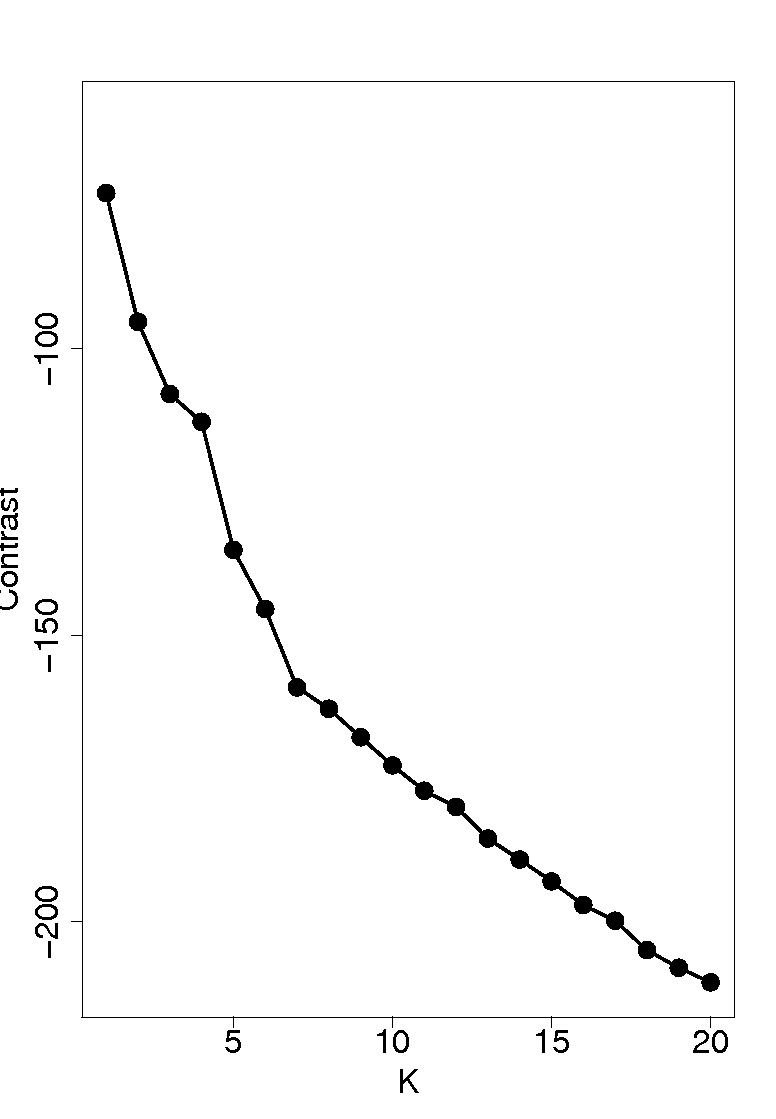
\epsfig{file = ../Figures/Bt474-J.ps, clip=, width=.5\textwidth,
	       height=.7\textheight} 
    	\onslide<3>
	      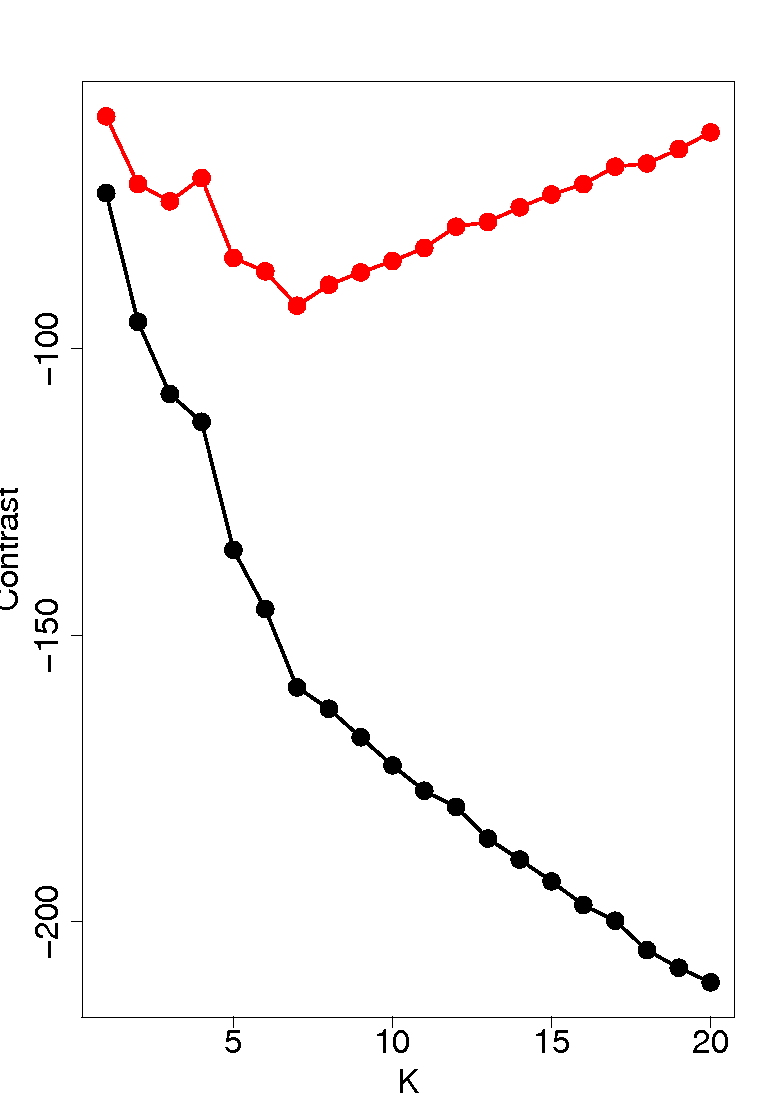
\epsfig{file = ../Figures/Bt474-JP.ps, clip=, width=.5\textwidth,
	       height=.7\textheight} 
    	\onslide<4->
	      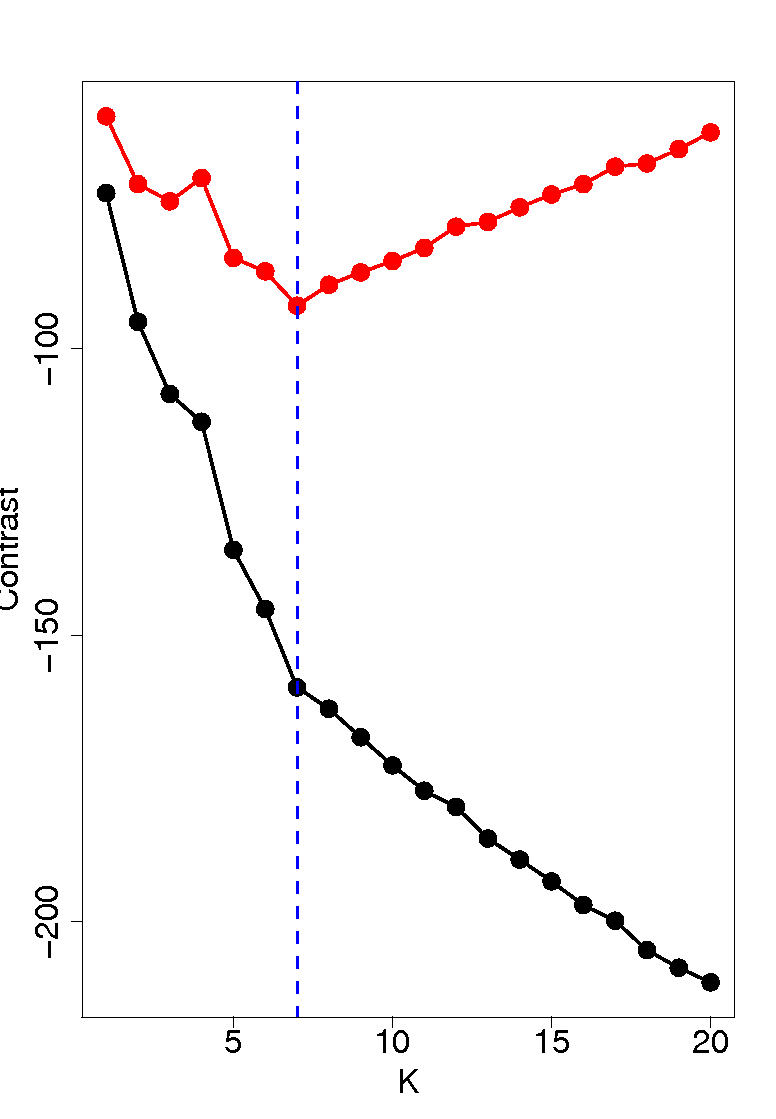
\epsfig{file = ../Figures/Bt474-JPM.ps, clip=, width=.5\textwidth,
	       height=.7\textheight} 
	    \end{overprint}
    \end{tabular} 
  \end{tabular} 

  \onslide+<5>{ 
    \vspace{-.5cm} A huge literature has been developed
    (\refer{Leb05}, \refer{Lav05}, \refer{ZhS07}, ...) to insure that
    $\Pr\{\widehat{K} = K\} \rightarrow 1$ when $n \rightarrow \infty$
    or to approximate $P(K | \Ybf)$.  }
  
}

%====================================================================
\frame{\frametitle{Speeding-up dynamic programming}

  \paragraph{Quadratic complexity} $O(Kn^2)$ is not acceptable for very
  large signals (e.g. NGS for DNAseq where $n = 10^6$ to $10^8$.

  \pause
  \begin{tabular}{cc}
    \hspace{-.75cm}
    \begin{tabular}{p{.5\textwidth}}
      \begin{itemize}
      \item \emphase{'Pruned DP'} can strongly reduce the
        computational burden (\refer{Rig10}).
      \item Its theoretical worst complexity is the same as regular
        DP.
      \item Its mean empirical complexity is \emphase{$O(K n \log n)$}.
      \end{itemize} 
      \emphase{R package available} \\
    \end{tabular}
    &
    \hspace{-.5cm}
    \begin{tabular}{p{.5\textwidth}}
    \epsfig{file = ../Figures/Rig10-Fig.ps, clip=, bbllx=290,
      bblly=20, bburx=560, bbury=270, width=.4\textwidth}     
    \end{tabular}
  \end{tabular}

  \pause
  \paragraph{Trick.} 
  Not to compute parameter estimates $\widehat{\Theta}$ (see \#
  \ref{Page:ParamInfer}) before to perform segmentation.  \\ \ra Only
  applicable for 'nice' models (e.g. Gaussian, Poisson, negative
  binomial with known $\phi$, ...)  }

%====================================================================
\frame{\frametitle{Breast cancer data (collab. Curie/Servier)}

  \vspace{-.5cm}
  \[
  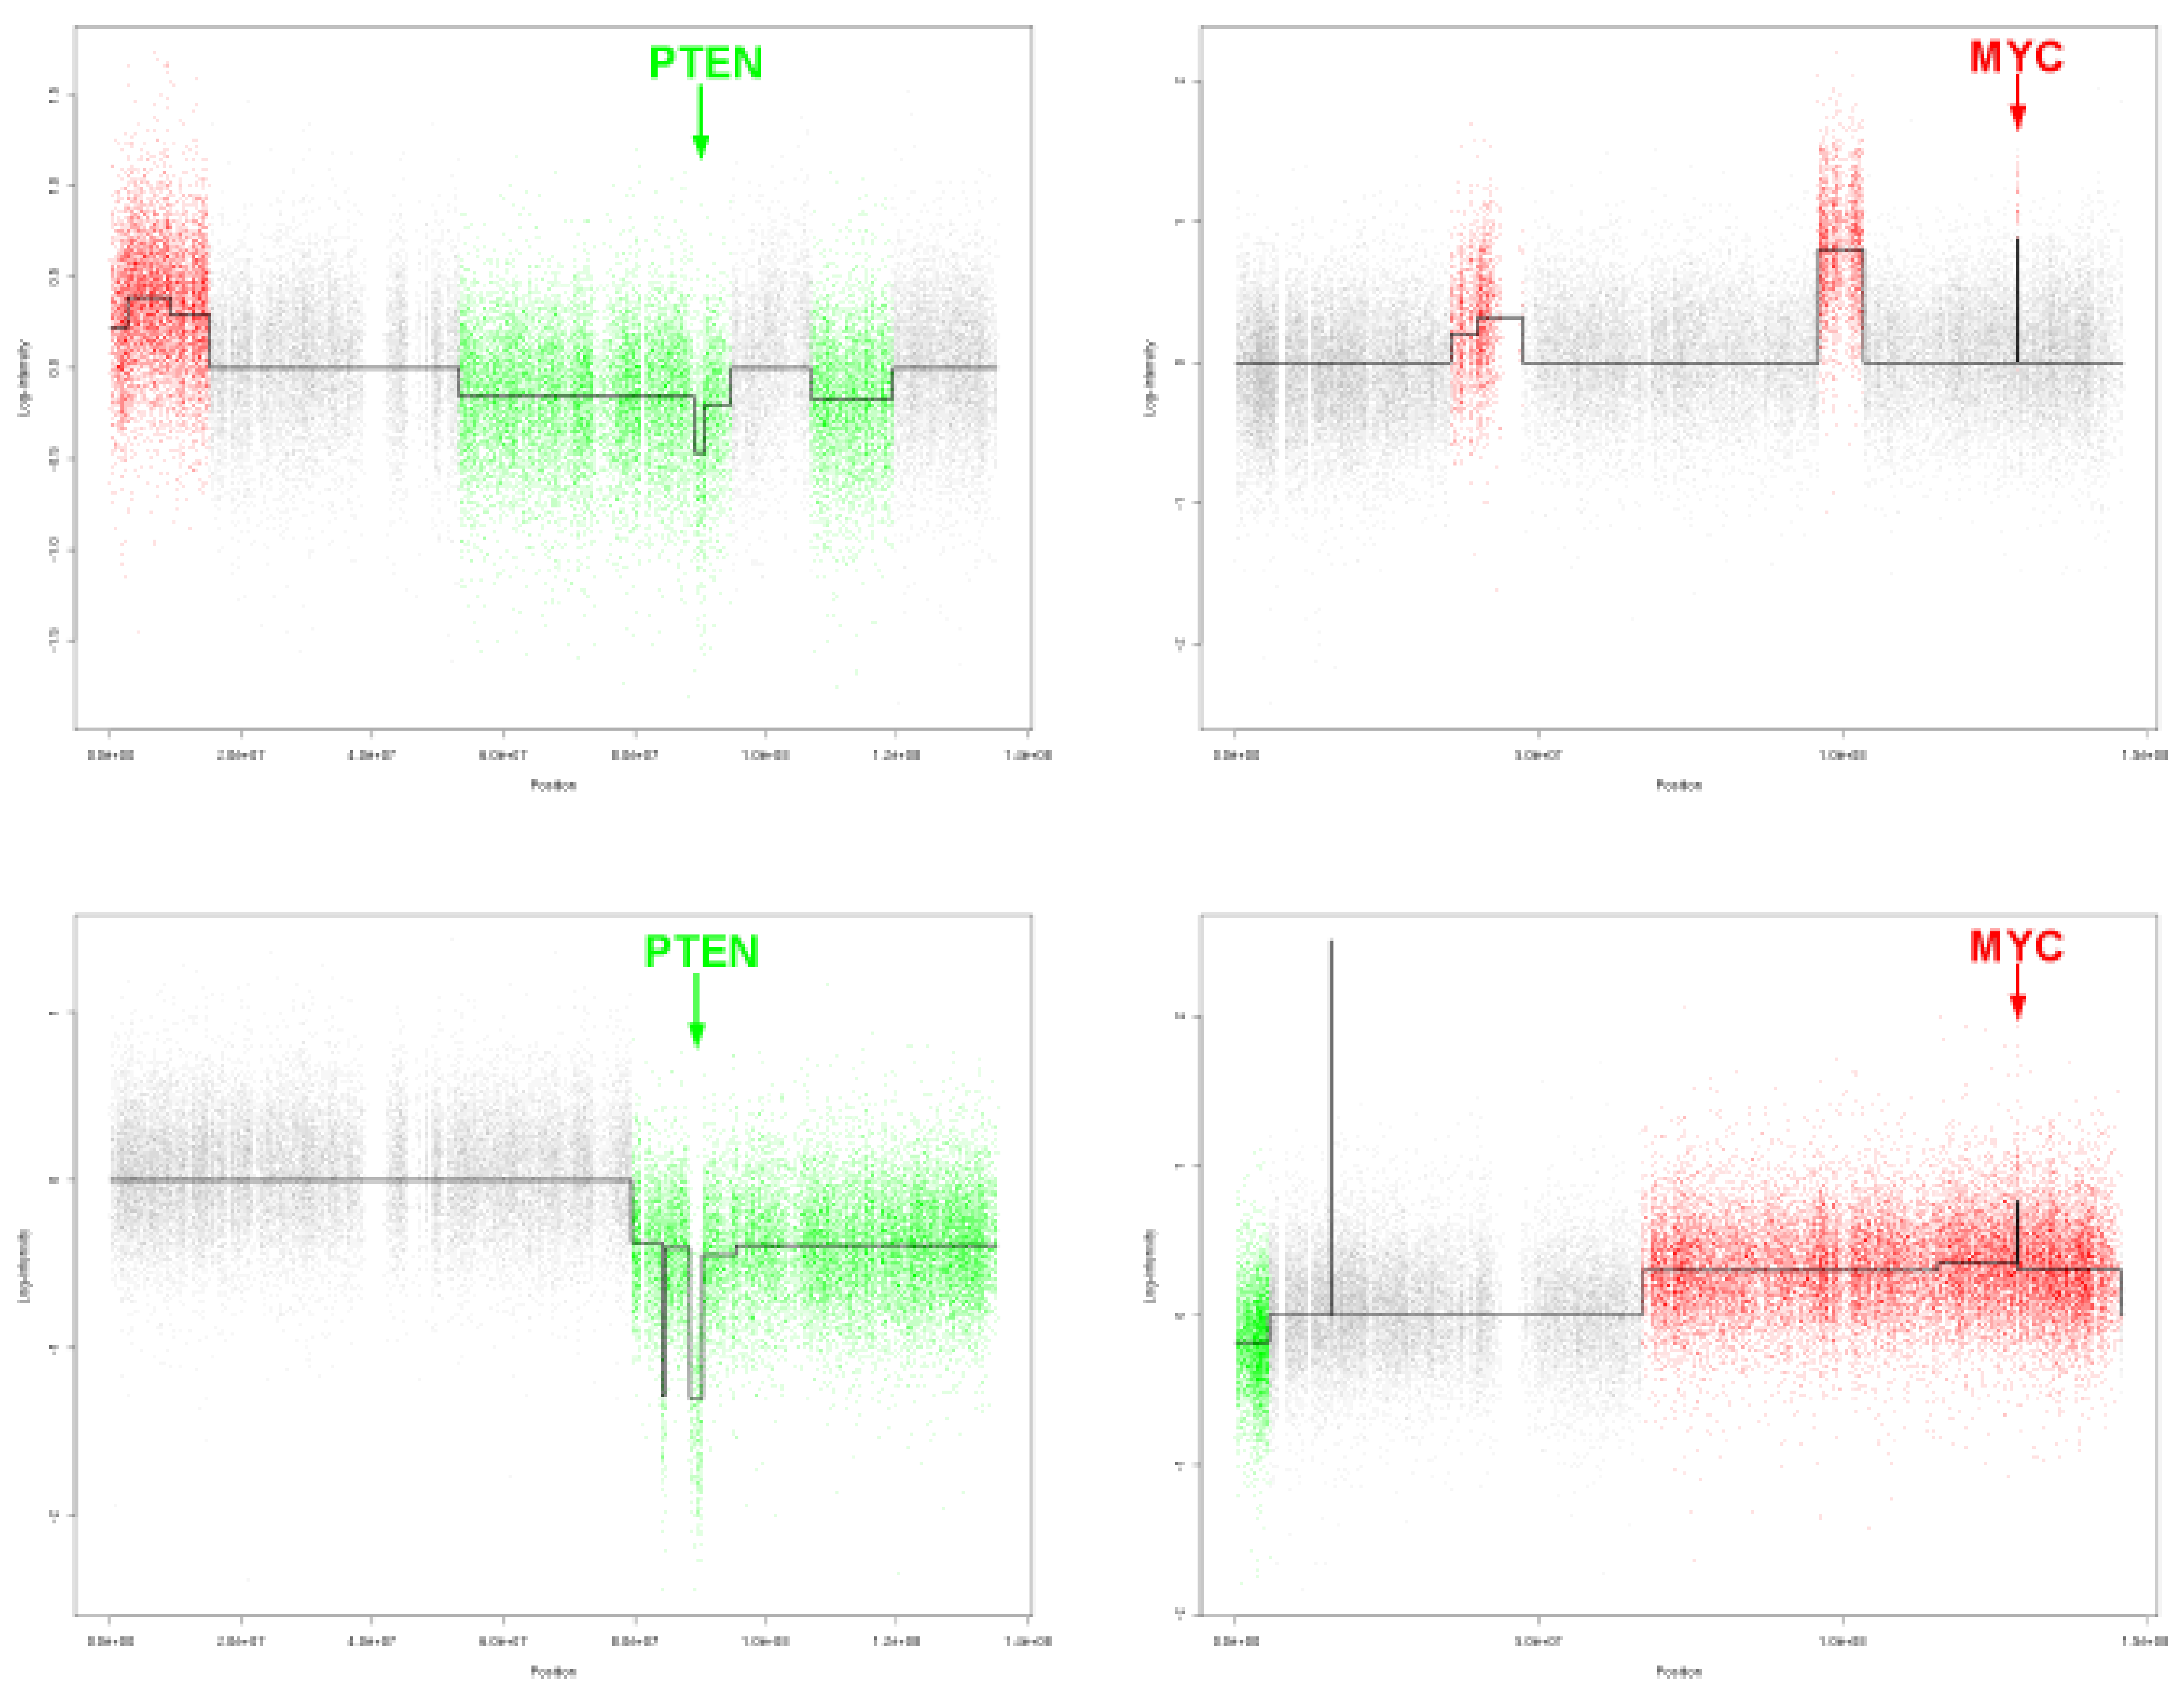
\epsfig{file = ../Figures/Rig10-Fig6-5.ps, height=.8\textheight,
    width=.8\textwidth} 
  \] 
  Chrom. 10 and 8 of two breast carcinomas (TNBC). \refer{Rig11} 
}\label{Page:BreastCancer}

%====================================================================
\subsection{Several Profiles}
%====================================================================
\frame{\frametitle{Several profiles}

    \begin{tabular}{cc}
    \begin{tabular}{p{.5\textwidth}}
      Cancer studies are most often carried on cohorts involving
      numerous CGH profiles ($m \approx 100$). \\
      \bigskip\pause
      The goal is then to detect recurrent alterations among patients
      carrying the same type of cancer.\\
      \bigskip
      As all the profiles are obtained with the same technology:
      \begin{itemize}
      \item same CGH probes, 
      \item same NGS sequences,
      \end{itemize}
      \emphase{correlations between profiles} are likelily to exist. 
      %\bigskip
      \refer{PLB11}
    \end{tabular}    
    &
    \begin{tabular}{p{6cm}}
      \hspace{-.75cm}
      \epsfig{file = ../Figures/nakao-mat.txt-MixSeg-V2.eps, bbllx=90,
      bblly=220, bburx=380, bbury=590, clip=, scale=.5}
    \end{tabular}
  \end{tabular}

}

%====================================================================
\frame{\frametitle{Algorithmic issue}

  \begin{tabular}{cc}
    \hspace{-.5cm}
    \begin{tabular}{p{.4\textwidth}}
      %\vspace{-1cm}      
      \onslide+<1->{\paragraph{One profile:} 
        OK with classical DP. \\}
      \onslide+<2->{\medskip
        \paragraph{Independent profiles:}
        OK with 2-stage DP. \\}
      \onslide+<3->{\medskip
        \paragraph{Correlation, same change points:} 
        same complexity as for one profile \ra classical DP. \\}
      \onslide+<4->{\medskip
        \paragraph{Correlation, different change points:} 
        Non-additivity of the likelihood \ra DP cannot apply as
        such.}
    \end{tabular}
    & 
    \hspace{-.5cm}
    \begin{tabular}{p{.5\textwidth}}
      \paragraph{Graphical model representation.} \\
      ~\\
      %\vspace{1cm}      
      \begin{overprint}
        \onslide<1>
        \epsfig{file=../Figures/SegFA-ModGraph-X1.eps, clip=,
          width=0.7\textwidth}
        \onslide<2>
        \epsfig{file=../Figures/SegFA-ModGraph-X1m.eps, clip=,
          width=0.7\textwidth}
        \onslide<3>
        \epsfig{file=../Figures/SegFA-ModGraph-XcovSimult.eps, clip=,
          width=0.7\textwidth}
        \onslide<4>
        \epsfig{file=../Figures/SegFA-ModGraph-Xcov.eps, clip=,
          width=0.7\textwidth}
%        \onslide<5>
%        \epsfig{file=../Figures/SegFA-ModGraph-Xcov.eps, clip=,
%          width=0.7\textwidth}
      \end{overprint}
    \end{tabular}
  \end{tabular}  

}

%====================================================================
\frame{\frametitle{Modeling the dependency}

  \paragraph{Joint segmentation model.} 
  In the Gaussian framework, we can write
  \[ 
  Y_{tm} = \mu_{km} + F_{tm}, \qquad \forall t \in
  r_k^{\emphase{m}}
  %\qquad \Fbf_t \text{ \emphase{i.i.d.} } \sim \Ncal_M(\Obf,
  %\emphase{\Sigmabf}).
  \]
  
  \bigskip\pause
  \paragraph{Factor model (Random effect model).} 
  An old trick in multivariate Gaussian models:
  \begin{itemize}
  \item \pause a (\emphase{unobserved}) random effect $\Zbf_t
    =(Z_{t1}, \dots, Z_{tQ}) \sim \Ncal(0, \Ibf)$ is associated to
    each position (probe);
  \item the residual terms $\Fbf_t$ at position $t$ all depend
    on this effect:
    \[
    \Fbf_t = \Bbf \Zbf_t + \Ebf_t, 
    \qquad \{\Ebf_t\} \text{ i.i.d. } \Ncal(0, \sigma^2 \Ibf);
    \]
  \end{itemize}
  \pause so the residuals at position $t$ have covariance matrix
  \[
  \Sigmabf = \Bbf \Bbf' + \sigma^2 \Ibf.
  \]
  
  \bigskip\bigskip 
  \ra This allows to capture any covariance structure
  (e.g. taking $Q = m-1$) 

}

%====================================================================
\frame{ \frametitle{Breaking down dependency}
  
  %\vspace{-1cm}      
  \begin{tabular}{cc}
    \hspace{-.5cm}
    \begin{tabular}{p{.4\textwidth}}
      \onslide+<1->{\paragraph{Marginal likelihood:} \\ $\log p(\Ybf)$ is
        not additive w.r.t. the segments $r_k^m$. \\}
      \onslide+<2->{\bigskip
        \paragraph{Joint likelihood:} $\log p(\Ybf, \Zbf)$ is
        still not additive. \\}
      \onslide+<3->{\bigskip
        \paragraph{Conditional likelihood:} \\
        $\log p(\Ybf|\Zbf)$ is additive w.r.t. the segments. \\  ~\\} 
    \end{tabular}
    & 
    \hspace{-.5cm}
    \begin{tabular}{p{.5\textwidth}}
      \vspace{1cm}      
      \begin{overprint}
        \onslide<1>
        \epsfig{file=../Figures/SegFA-ModGraph-Xcov.eps, clip=,
          width=0.7\textwidth}
        \onslide<2>
        \epsfig{file=../Figures/SegFA-ModGraph-XZ.eps, clip=,
          width=0.7\textwidth}
        \onslide<3->
        \epsfig{file=../Figures/SegFA-ModGraph-XcondZ.eps, clip=,
          width=0.7\textwidth}
      \end{overprint}
    \end{tabular}
  \end{tabular}
  
%  \onslide+<4>{
%    \vspace{-1.25cm}
%    \paragraph{E-M algorithm:} Dynamic programming can be applied
%    within the M step, when maximizing
%    \[
%    \Esp[\log P(\Ybf, \Zbf) | \Ybf].
%    \]
%  }
  
}

%====================================================================
\frame{ \frametitle{E-M algorithm}

  \paragraph{Incomplete data model.} 
  In the factor model, the random effect $\Zbf$ is unobserved.

  \bigskip\pause
  \paragraph{E-M algorithm.} To perform maximum likelihood inference:
  \[
  (\widehat{T}, \widehat{\Theta}, \widehat{\Sigma}) = \arg\max_{T, \Theta} \; \log
  P(\Ybf; T, \Theta, \Sigma) 
  \]
  first notice that
  \[
  \log P(\Ybf; T, \Theta) = \Esp[\log P(\Ybf, \Zbf; T, \Theta) | \Ybf]
  - \Esp[\log P(\Zbf | \Ybf; T, \Theta) | \Ybf] \pause
  \]
  then, iteratively,
  \begin{itemize}
  \item \paragraph{E-step:} compute the conditional distribution
    $P(\Zbf | \Ybf; \widehat{T}, \widehat{\Theta}, \widehat{\Sigma})$;
  \item \paragraph{M-step:} update the estimates as
    \begin{eqnarray*}
      (\widehat{T}, \widehat{\Theta}, \widehat{\Sigma}) & = &
      \arg\max_{T, \Theta} \; \Esp[\log P(\Ybf, \Zbf; T, \Theta,
        \Sigma) | \Ybf] \\ 
      & = & \arg\max_{T, \Theta} \; \Esp[\log P(\Zbf; \Sigma) | \Ybf]
      + \Esp[\log P(\Ybf| \Zbf; T, \Theta) | \Ybf]
    \end{eqnarray*}
... which can be achieved with dynamic programming.
  \end{itemize}
  }
  
%====================================================================
\frame{ \frametitle{Bladder cancer data (collab. Curie)}
  
  \vspace{-.5cm}
  \begin{tabular}{cc}
    \begin{tabular}{p{5cm}}
      \onslide+<1->{
        Some large probe effect $Z_t$ are detected\\
        $\rightarrow$ \emphase{Poor probe affinity}? \\
        $\rightarrow$ \emphase{Wrong annotation}? \\
        $\rightarrow$ \emphase{Polymorphism}? \\
      }
      \onslide+<2->{
        \bigskip
        Breakpoints near this position are likely to be artifacts. \\
        }
      \onslide+<3->{
        \bigskip
        The global segmentation is affected by this correction:\\
        \textcolor{red}{--}: independent segmentation, \\
        --: multivariate mixed segmentation.
        }
    \end{tabular}
    &
    \hspace{-1cm}
    \begin{tabular}{c}
      \onslide+<1->{
        \hspace{.1cm}\epsfig{file= ../Figures/random_effect.ps, clip=, 
          width=3cm, height=6.7cm, angle=270} \\
      }
      \onslide+<2->{
        \epsfig{file= ../Figures/profils2_9_29.ps, width=6cm,
          height=2.5cm, clip=, bbllx=90, bblly=490, bburx=490, bbury=605} \\
      }
      \onslide+<3->{
        \hspace{.1cm}\epsfig{file= ../Figures/profils2_9_29.ps, width=6cm,
          height=2.5cm, clip=, bbllx=90, bblly=210, bburx=490, bbury=335} 
        }
    \end{tabular}
  \end{tabular}

  }

%====================================================================
\subsection*{CGH-seg package}
%====================================================================
\frame{\frametitle{CGH-seg package}

  \paragraph{CGHseg} is an R package dedicated to the analysis of
  CGH profiles \refer{PLH11}.
  
  \bigskip\pause
  \paragraph{Linear model framework:} 
 
  \medskip
  \begin{tabular}{p{.2\textwidth}p{.35\textwidth}p{.35\textwidth}}
%     \emphase{Task} & \emphase{Representation} & \emphase{Model} \\   
%     \hline
%     \\
    \emphase{Segmentation} & regression on unknown $\Tbf$: &
    $\displaystyle{\Ybf = \Tbf \mubf + \Ebf}$ \pause \\ 
    \\
    \emphase{Correlation} & {Factor model(\footnote{uniform
        correlation}): $\Zbf$}  & 
    $\displaystyle{\sl \Ybf = \Tbf \mubf + \Bbf \Zbf + \Ebf}$ \pause \\ 
    \\
    \emphase{Correction} & fixed covariates effect: $\betabf$ &
    $\displaystyle{\Ybf = \Tbf \mubf + \Xbf \betabf + \Ebf}$ \pause \\  
    \\
    \emphase{Calling} & crosstabulation table $\Cbf$: &
    $\displaystyle{\Ybf = \Tbf \Cbf \mbf + \Ebf}$ \pause \\
    \\
    \emphase{Combinations} 
    & fixed + random effects: &
    $\displaystyle{\Ybf = \Tbf \mubf + \Xbf \betabf + \Lbf \Zbf + \Ebf}$ \\
    & fixed effects + calling: &
    $\displaystyle{\Ybf = \Tbf \Cbf \mbf + \Xbf \betabf + \Ebf}$  \\
  \end{tabular}
}

%====================================================================
%====================================================================
\section{Bayesian inference}
%====================================================================
\frame{\frametitle{Bayesian framework} \pause

  \paragraph{Limitation of the frequentist approach:} 
  Due the discrete nature of the change points, their inference is
  complex and \emphase{confidence intervals} can not been easily derived.

  \bigskip\bigskip\pause
  \paragraph{Bayesian principle:} 
  All parameters ($K$, $T$, $\Theta$) are random.
  \begin{itemize}
  \item \emphase{Prior} distribution of the parameters: $P(K)$,
    $P(T|K)$, $P(\Theta|T, K)$;
  \item \emphase{Likelihood} of the data given the parameters: $P(\Ybf
    | K, T, \Theta)$;
  \item \emphase{Posterior} distribution of the parameter:
    \[
    P(K, T, \Theta | \Ybf) = \frac{P(K, T, \Theta, \Ybf)}{P(\Ybf)} \pause
    \]
    where
    \begin{eqnarray*}
      P(K, T, \Theta, \Ybf) & = & P(K) P(T|K) P(\Theta|T, K) (\Ybf |
      K, T, \Theta) \\ 
      P(\Ybf) & = & \sum_K \sum_{T \in \Mcal_K} \int_\Theta P(K, T,
      \Theta, \Ybf).
    \end{eqnarray*}
  \end{itemize}
}

%====================================================================
\frame{\frametitle{Posterior distributions}

  \paragraph{Biological questions:}  
  \begin{itemize}
  \item \pause How many change points? \ra $P(K | \Ybf)$;
  \item \pause Where are the change points?  \ra $P(T | \Ybf, K)$ or
    $P(T | \Ybf)$;
  \item \pause How precise is the location?  \ra $P(\tau_1 | \Ybf, K)$
    or $P(\tau_1 | \Ybf)$;
  \item \pause Do the change points have the same location in samples
    $A$ and $B$? \\ \ra $P(\tau_1^A - \tau_1^B | \Ybf^A, \Ybf^B)$.
  \end{itemize}

  \bigskip\pause
  \paragraph{One common issue.} 
  The calculation of most of these quantities requires to \emphase{sum
    over the whole segmentation space}, e.g.
  \[ 
  P(\Ybf | K) = \sum_{T \in \Mcal_K} P(\Ybf, T | K)  
  \]
  where $\Mcal_K$ stands for the set of all $K$-segment segmentations.
  }

%====================================================================
\subsection*{Exact posterior}
%====================================================================
\frame{\frametitle{Calculating exact posterior distributions}
  \paragraph{1 - Factorization assumption:}
  \[
  P(T) = \prod_{r \in T} f(r), 
  \quad
  P(\theta|T) = \prod_{r \in T} f(\theta_r) 
  \quad
  P(\Ybf|T, \theta) = \prod_{r \in T} f(Y^r, \theta_r)  \pause
  \]

  \paragraph{2 - Conjugate prior:}
  \[
  \int P(Y^r | \theta_r) P(\theta_r) \dd \theta_r 
  \quad
  \text{has a closed form expression.}
  \]

  \bigskip\pause
  \paragraph{Sum-product form:} The total probability can be rewritten as 
  \begin{eqnarray*}
  P(\Ybf|K) & = & \sum_{T \in \Mcal_K} \int_\Theta P(\Ybf, T, \Theta | K) \\
  & = & \sum_{r \in \Mcal_K} \prod_{r \in T} P(Y^r)
  \end{eqnarray*}

%  \pause
%  \paragraph{Localisation of the $k$-th breakpoint:}
%  \begin{eqnarray*}
%    \Pr\{\tau_k = t | K, \Ybf\} & \propto & \left(\sum_{r \in \Mcal_k(1, t)} \prod_{r
%    \in T} P(Y^r)\right) \left(\sum_{r \in \Mcal_{K-k}(t+1, n)} \prod_{r
%    \in T} P(Y^r)\right)
%  \end{eqnarray*}
%   \emphase{Conjugate priors.} $\theta^0_r =$ parameter
%     of the prior $P(\theta_r)$
%     \[
%     f(Y^r; \theta^0_r) = \int P(Y^r|\theta_r) P(\theta_r; \theta^0_r) 
%         \dd \theta_r
%     \quad \text{has an explicit form.}
%     \]
%     Avoids the Laplace approximation: \\
%     $\rightarrow$ regularity conditions \emphase{are fulfilled} for
%     any segmentation $T$, \\
%     $\rightarrow$ but the asymptotic framework does not apply to small regions.
  }

%====================================================================
\frame{ \frametitle{Exploring the segmentation space}

  \paragraph{Computational consequence.}
  $\sum_{r \in \Mcal_K} \prod_{r \in T} P(Y^r)$ can be computed as
  \[
  [\Abf^K]_{0, n}, \qquad \text{where } A_{ij} = P(Y_{i+1}, \dots Y_j);
  \]
  with complexity \emphase{$O(Kn^2)$} \refer{RLR11}.

  \bigskip\pause
  We are hence able to compute with quadratic complexity, \pause
  \begin{itemize}
  \item The probability that there is a \emphase{breakpoint at
      position $t$};
  \item The probability for a \emphase{segment $r = \llbracket t_1,
      t_2 \llbracket$ to be part of segmentation};
  \item The \emphase{posterior entropy of $T$} within a dimension;
  \end{itemize}   \pause
  \paragraph{Similar to} an algorithm proposed by \refer{Gue07} in the HMM
  context with known parameters.

  \bigskip\pause
  \paragraph{Algorithmic comment.}
  Replacing products with sums and sums with 'min' gives the dynamic
  programming algorithm mentioned in \# \ref{Page:ParamInfer}.

 }

%====================================================================
\frame{ \frametitle{An computational remark}

  \paragraph{Optimal segmentation.} To obtain
  \[
  L_K(Y_1^n) = \textcolor{blue}{\max_{T \in \Mcal_K}}
  \textcolor{red}{\sum_{r_k \in T}} \log p(Y^{r_k}),
  \]
  we use the dynamic programming recursion
  \[
  L_{K+1}(Y_1^j) = \textcolor{blue}{\max_i} \; L_K(Y_1^i)
  \textcolor{red}{+} \log p(Y_{i+1}^j).
  \]

  \bigskip\pause
  \paragraph{Posterior distribution.} To compute
  \[
  p(Y_1^n|K) = \textcolor{blue}{\sum_{T \in \Mcal_K}} \;
  \textcolor{red}{\prod_{r_k \in T}} p(Y^{r_k}),
  \]
  we use the matrix product:
  \[
  p(Y_1^j|K+1) = \textcolor{blue}{\sum_i} \; p(Y_1^i|K)
  \textcolor{red}{\times} p(Y_{i+1}^j|1).
  \]

  }

%====================================================================
\frame{ \frametitle{A CGH profile: $K = 3, 4$}
  
  \vspace{-.75cm}
  \[
  \begin{tabular}{ll}
    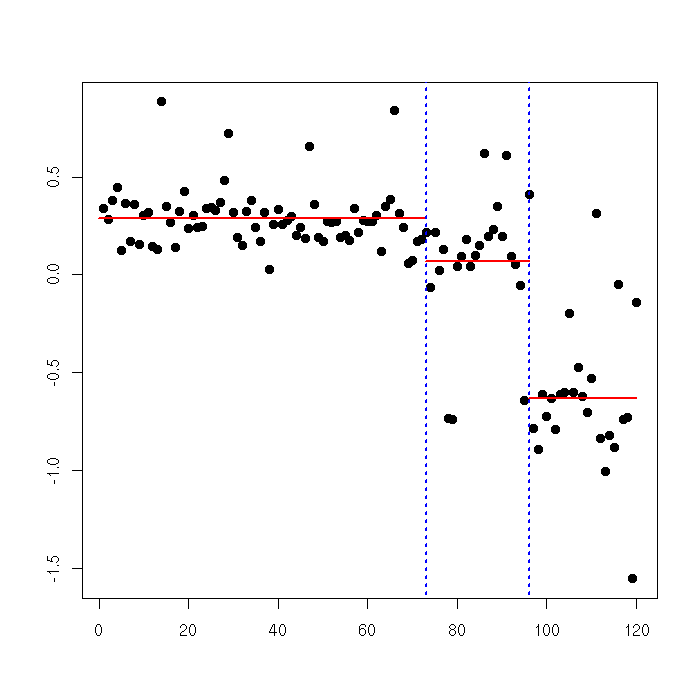
\includegraphics[width=0.45\textwidth, height=0.45\textheight,
      clip=]{\fighd/CopyNumberChr10_BIC} 
    &
    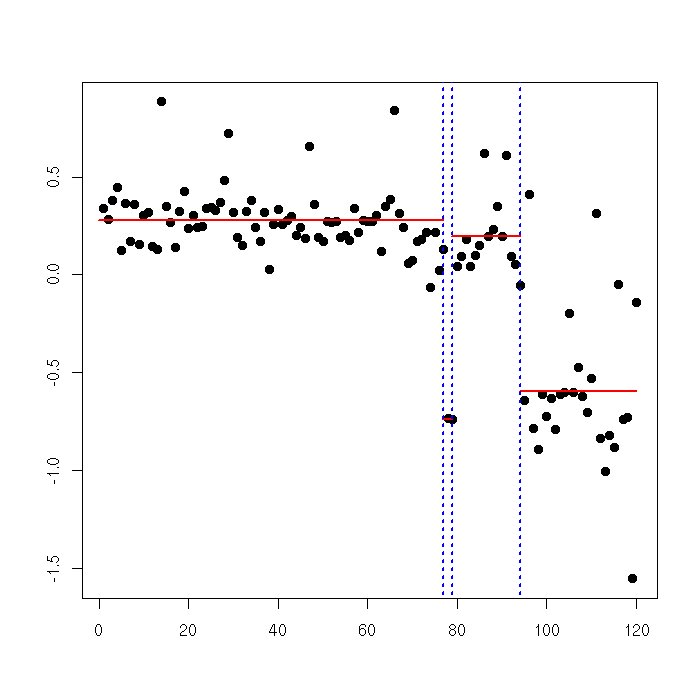
\includegraphics[width=0.45\textwidth, height=0.45\textheight,
      clip=]{\fighd/CopyNumberChr10_ICL} 
    \\
    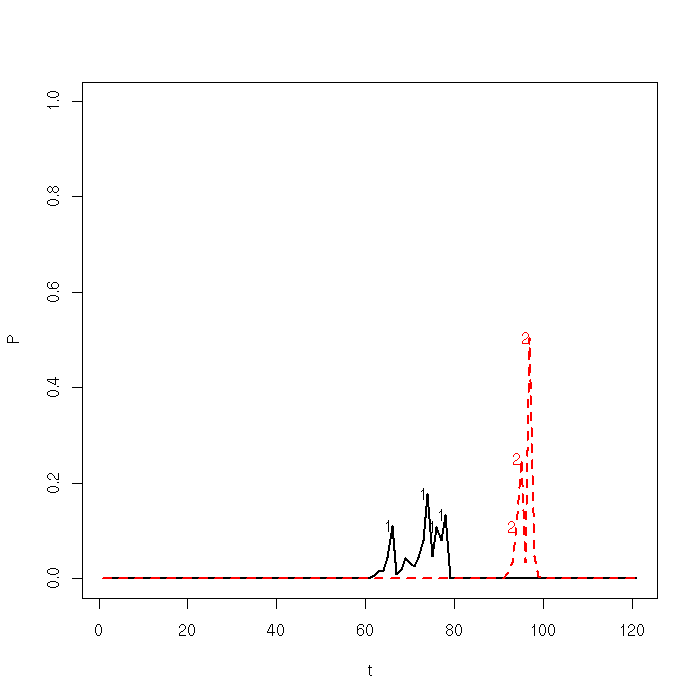
\includegraphics[width=0.45\textwidth, height=0.45\textheight,
      clip=]{\fighd/CopyNumberChr10_ProbaBIC}
    &
    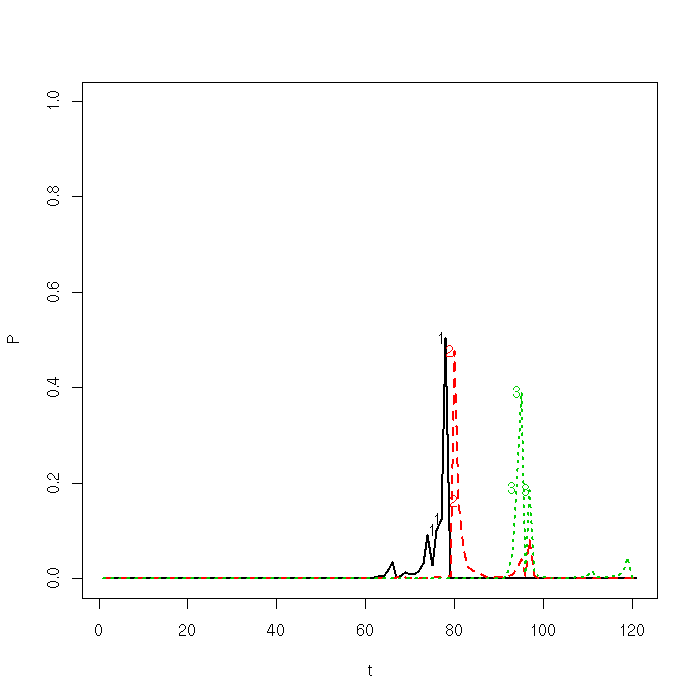
\includegraphics[width=0.45\textwidth, height=0.45\textheight,
      clip=]{\fighd/CopyNumberChr10_ProbaICL}  
  \end{tabular}
  \]

  }

%====================================================================
\frame{ \frametitle{Presence of an alteration}

  To assess the gain or loss of a given locus (e.g. gene), one need to
  know if it is included within an alteration (see slide \#
  \ref{Page:BreastCancer}). 

  \bigskip
  The posterior probability of a segment can be computed as well:
  \[
  f(t_1, t_2) = \Pr\{\exists k: r_k = \llbracket t_1, t_2 \llbracket |
  \Ybf, K\}
  \]
  
  \pause
  \[
  \begin{tabular}{cc}
    $K=3$ & $K=4$ \\
    \begin{tabular}{c}
      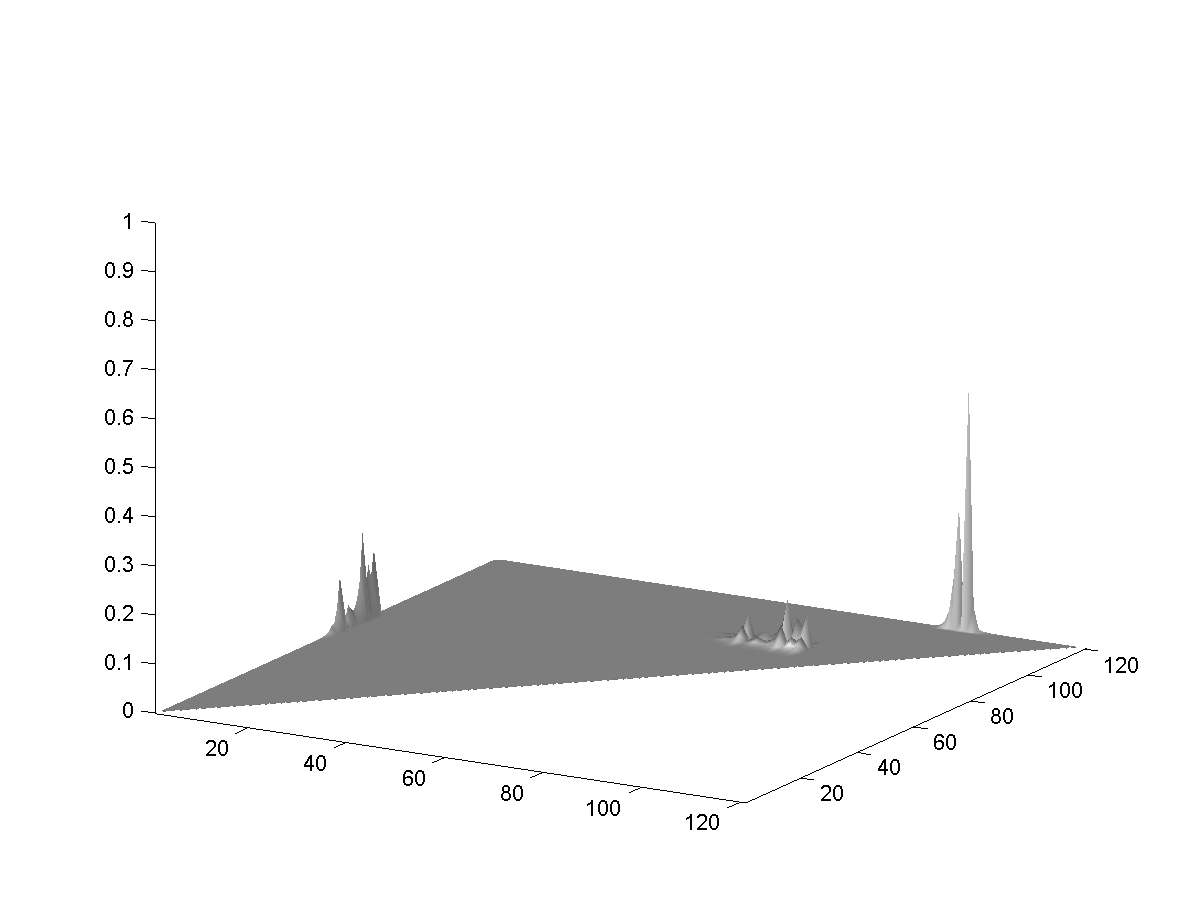
\includegraphics[width=0.5\textwidth, height=0.5\textheight,
        clip=]{\fighd/ProbSeg-BIC} 
    \end{tabular}
    &
    \hspace{-1cm}
    \begin{tabular}{c}
      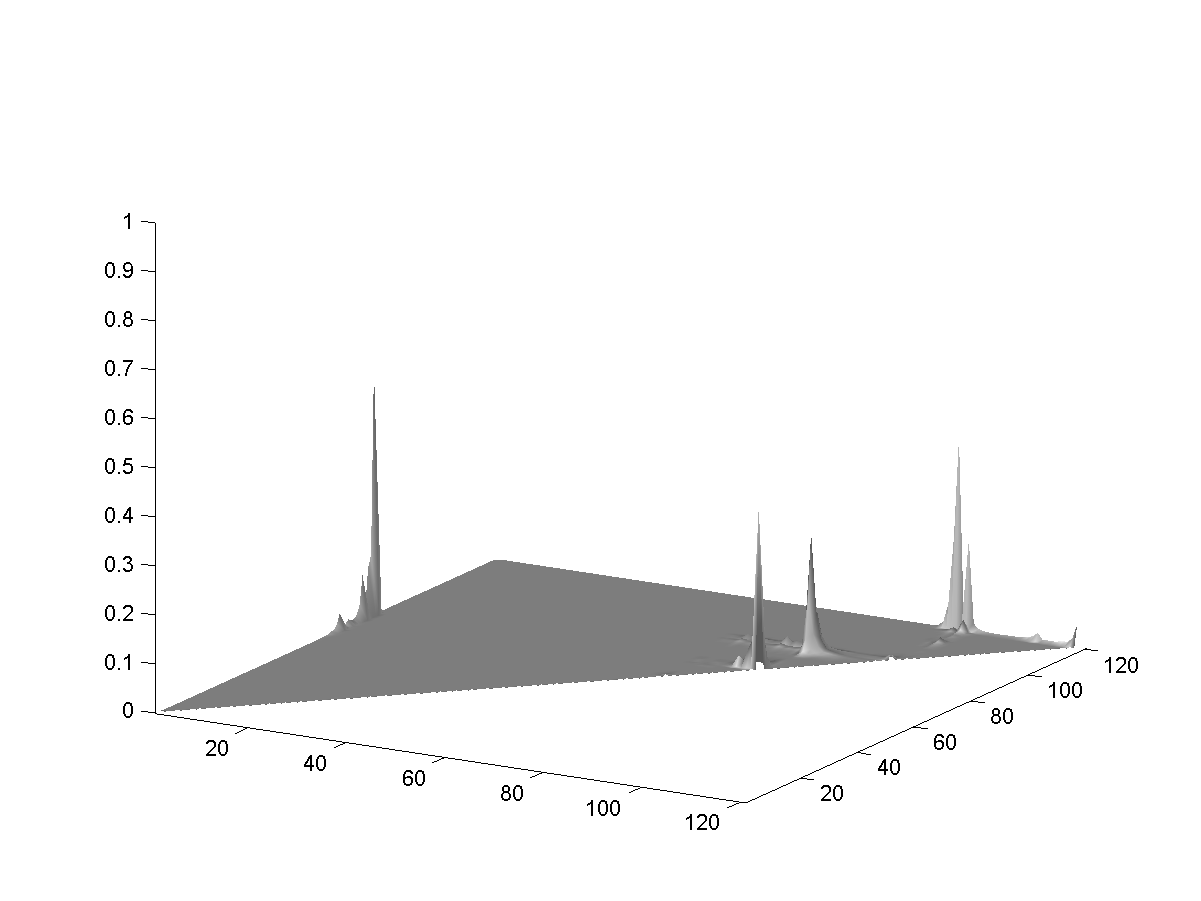
\includegraphics[width=0.47\textwidth, height=0.4\textheight,
        clip=]{\fighd/ProbSeg-ICL} \\
      ~ \\ ~
    \end{tabular}
  \end{tabular}
  \]

}

%====================================================================
\frame{ \frametitle{Model selection: exact BIC and ICL}

  Standard model selection criteria can be computed exactly (without,
  say, Laplace approximation).

  \bigskip
  \paragraph{Choice of $K$.} Exact version of $\BIC(K)$:
  \[
  \log P(\Ybf, K) 
%  = \log \left[\emphase{\sum_{r \in \Mcal_K}} P(T) \int P(\Ybf | T,
%    \theta) P(\theta |T) \dd \theta \right].
  \]
  \pause
  \paragraph{Choice of $T$.} Exact version of $\BIC(T)$:
  \[
  \log P(\Ybf, T) 
%  = \log \left[P(T) \int P(\Ybf | T, \theta) P(\theta |T) \dd \theta
%    \right]
  \]
%  where $P(T)$ must be normalised so that
%  \[
%  \sum_K \emphase{\sum_{r \in \Mcal_K}} P(T) = 1.
%  \]
  \pause
  \paragraph{Alternative choice of $K$.} Exact version of $\ICL(T)$ (\refer{BCG00}):
  \[
  \log P(\Ybf, K) + \underset{\text{-- Entropy within
    $\Mcal_K$}}{\underbrace{\sum_{r \in \Mcal_K} P(T|\Ybf, K) \log
      P(T|\Ybf, K)}}
%  = \log \left[\emphase{\sum_{r \in \Mcal_K}} P(T) \int P(\Ybf | T,
%    \theta) P(\theta |T) \dd \theta \right].
  \] 
  favors dimensions $K$ the best segmentation $\widehat{T}_K$ clearly
  outperforms the others.

  }

%====================================================================
\frame{ \frametitle{Comparison BIC/ICL: simulation study}
  \begin{columns}
    \begin{column}{0.45\linewidth}
      \emphase{Simulations: } Poisson signal with alternating
      means $\lambda_0$ and $\lambda_1$, $n = 100$. \\
      \bigskip \emphase{Criterion} = \% of recovery of the true number
      of segments ($K =
      5$). \\
      \bigskip
      \begin{itemize}
      \item $\BIC(T)$ achieves (much) better performances than
        $\BIC(K)$
      \item $\ICL(K)$ outperforms both $\BIC(K)$ and $\BIC(T)$.
      \end{itemize}
    \end{column}
    
    \begin{column}{0.45\linewidth}
      \begin{tabular}{c}
        \textcolor{green}{$\BIC(K)$} \quad \textcolor{red}{$\BIC(T)$} \quad
        \textcolor{blue}{$\ICL(K)$} \\
        ~\\
        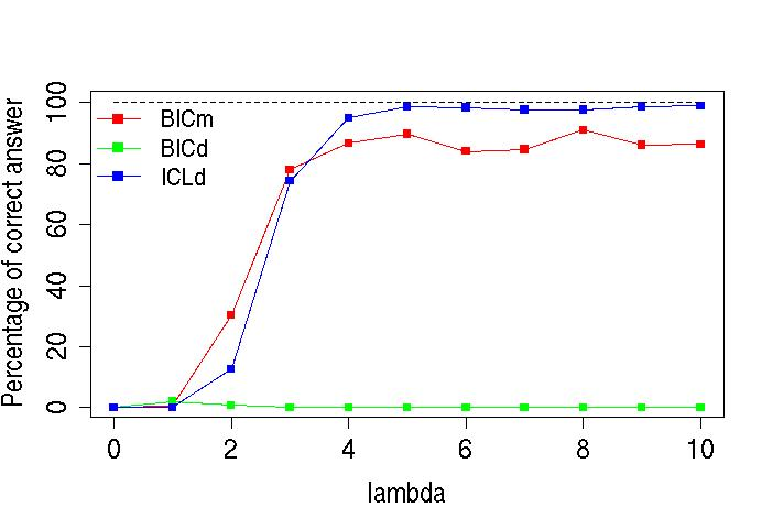
\epsfig{file=\fighd/ICLvsBIC.ps, clip=, bbllx=50, bblly=60,
          bburx=545, bbury=340, width=.9\textwidth,
        height=.5\textheight} \\ 
        $\lambda_1 - \lambda_0$ ($\lambda_0 = 1$) \\
        \\
        \refer{RLR11}
      \end{tabular}
    \end{column}
  \end{columns}
 }


%====================================================================
\subsection*{Alternative splicing}
%====================================================================
\frame{\frametitle{Re-annotation}

  \vspace{-0.5cm}
  \begin{tabular}{cc}
    \hspace{-0.5cm}
    \begin{tabular}{p{.45\textwidth}}
      The posterior distribution of the change-points location can be
      used to assess the genome annotation.

      \bigskip
      It also allows to study variations of the transcription start
      due to condition changes.

      \bigskip
      \Refer{Cleynen (2012)}
    \end{tabular}
    &
    \begin{tabular}{p{.5\textwidth}}
      \epsfig{file=../Figures/Bayes-data.ps, clip=, width=0.5\textwidth}
    \end{tabular}
  \end{tabular}

}

%====================================================================
\frame{\frametitle{Alternative splicing (collab. univ. Berkeley)}

  \vspace{-0.5cm}
  \begin{tabular}{cc}
    \hspace{-0.5cm}
    \begin{tabular}{p{.5\textwidth}}
      Alternative splicing refer to modification of exon boundaries
      (or to exon skipping).

      \bigskip
      Based on the posterior distribution of exon boundaries, a 'test'
      for alternative splicing can be derived. \\
      ~\\~\\
    \end{tabular}
    &
    \hspace{-1cm}
    \begin{tabular}{p{.5\textwidth}}
      \epsfig{file=../Figures/compa-end.ps, clip=, bbllx=0, bblly=0,
        bburx=520, bbury=210, width=0.5\textwidth, height=0.5\textheight}
    \end{tabular}
  \end{tabular}

  \pause
  The \emphase{EBS package} performs an exact bayesian segmentation on data and
  returns all quantities described above:
  \[
  \text{cran.r-project.org/web/packages/EBS}
  \]
}

%====================================================================
\frame{\frametitle{Discussion}

  \paragraph{Statistics} 
  are needed to assess the existence and the location of genomic
  alteration or to comfort genome annotation.

  \bigskip\pause
  \paragraph{Algorithmic} 
  complexity is one major limitation of such analyses. \\ 
  \ra How to manage profiles on $10^8$ nucleotides for a cohort of
  $10^3$ or $10^4$ patients?

  \bigskip\pause
  \paragraph{Some related questions.}
  \begin{itemize}
  \item Assess the relation between an alteration with given 
    length and frequency in a cohort an a certain type of cancer.
  \item Study the influence of various experimental conditions on
    alternative splicing for genes with a large (10, 20) number of
    exons.
  \end{itemize}
  }

%====================================================================
\frame{\frametitle{Acknowledgment}
  
  \paragraph{Some of the co-authors:}
  \begin{itemize}
  \item E. Lebarbier, A. Cleynen (AgroParisTech/INRA)
  \item F. Picard (CNRS, LBBE, Lyon)
  \item F. Radvanyi (Institut Curie)
  \item G. Rigaill (Univ. Evry, INRA-URGV)
  \end{itemize}
  
}

%====================================================================
\section*{Appendix}
%====================================================================
{\tiny
  \bibliography{/media/donnees/Biblio/ARC,/media/donnees/Biblio/AST,/media/donnees/Biblio/SSB}
  \bibliographystyle{/media/donnees/LATEX/astats}
  %\bibliographystyle{plain}
  }

%====================================================================
%====================================================================
\end{document}
%====================================================================
%====================================================================


\frame{\frametitle{}
  }

  \vspace{-0.5cm}
  \begin{tabular}{cc}
    \hspace{-0.5cm}
    \begin{tabular}{p{.5\textwidth}}
    \end{tabular}
    &
    \hspace{-1cm}
    \begin{tabular}{p{.5\textwidth}}
    \end{tabular}
  \end{tabular}
